\documentclass[10pt,a4paper]{article}
\usepackage[UTF8,fontset = windows]{ctex}
\setCJKmainfont[BoldFont=黑体,ItalicFont=楷体]{华文中宋}
\usepackage{amssymb,amsmath,amsfonts,amsthm,mathrsfs,dsfont,graphicx}
\usepackage{ifthen,indentfirst,enumerate,color,titletoc}
\usepackage{tikz}
\usepackage{makecell}
\usepackage{longtable}

\usetikzlibrary{arrows,calc,intersections,patterns}
\usepackage[bf,small,indentafter,pagestyles]{titlesec}
\usepackage[top=1in, bottom=1in,left=0.8in,right=0.8in]{geometry}
\renewcommand{\baselinestretch}{1.65}
\newtheorem{defi}{定义~}
\newtheorem{eg}{例~}
\newtheorem{ex}{~}
\newtheorem{rem}{注~}
\newtheorem{thm}{定理~}
\newtheorem{coro}{推论~}
\newtheorem{axiom}{公理~}
\newtheorem{prop}{性质~}
\newcommand{\blank}[1]{\underline{\hbox to #1pt{}}}
\newcommand{\bracket}[1]{(\hbox to #1pt{})}
\newcommand{\onech}[4]{\par\begin{tabular}{p{.9\textwidth}}
A.~#1\\
B.~#2\\
C.~#3\\
D.~#4
\end{tabular}}
\newcommand{\twoch}[4]{\par\begin{tabular}{p{.46\textwidth}p{.46\textwidth}}
A.~#1& B.~#2\\
C.~#3& D.~#4
\end{tabular}}
\newcommand{\vartwoch}[4]{\par\begin{tabular}{p{.46\textwidth}p{.46\textwidth}}
(1)~#1& (2)~#2\\
(3)~#3& (4)~#4
\end{tabular}}
\newcommand{\fourch}[4]{\par\begin{tabular}{p{.23\textwidth}p{.23\textwidth}p{.23\textwidth}p{.23\textwidth}}
A.~#1 &B.~#2& C.~#3& D.~#4
\end{tabular}}
\newcommand{\varfourch}[4]{\par\begin{tabular}{p{.23\textwidth}p{.23\textwidth}p{.23\textwidth}p{.23\textwidth}}
(1)~#1 &(2)~#2& (3)~#3& (4)~#4
\end{tabular}}
\begin{document}
\begin{enumerate}[1.]

\item 函数$f(x)={x^{-\frac 12}}$的定义域是\blank{50}.
\item 集合$A=\{-1, 2m-1\}$, $B=\{m^2\}$, 若$B\subseteq A$, 则实数$m=$\blank{50}.
\item $(1+2x)^5=a_0+a_1x+a_2x^2+a_3x^3+a_4x^4+a_5x^5$, 则$a_3=$\blank{50}
\item 如图, 若正四棱柱$ABCD-A_1B_1C_1D_1$的底面边长为$3$, 高为$4$, 则直线$BD_1$与平面$ABCD$所成角的正切值为\blank{50}.
\begin{center}
    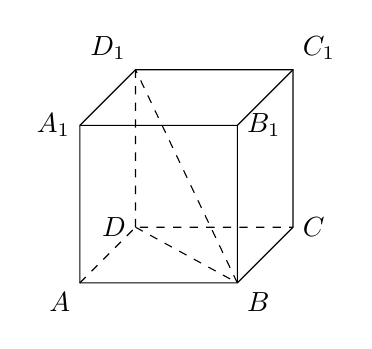
\begin{tikzpicture}
        \draw (0,0) node [below left] {$A$} coordinate (A) --++ (2,0) node [below right] {$B$} coordinate (B) --++ (45:{2/2}) node [right] {$C$} coordinate (C)
        --++ (0,2) node [above right] {$C_1$} coordinate (C1)
        --++ (-2,0) node [above left] {$D_1$} coordinate (D1) --++ (225:{2/2}) node [left] {$A_1$} coordinate (A1) -- cycle;
        \draw (A) ++ (2,2) node [right] {$B_1$} coordinate (B1) -- (B) (B1) --++ (45:{2/2}) (B1) --++ (-2,0);
        \draw [dashed] (A) --++ (45:{2/2}) node [left] {$D$} coordinate (D) --++ (2,0) (D) --++ (0,2);
        \draw [dashed] (D) -- (B) -- (D1);
    \end{tikzpicture}
\end{center}
\item 方程$\lg (x+2)=2\lg x$的解为\blank{50}.
\item 若$\arccos x>\dfrac{\pi}3$, 则$x$的取值范围为\blank{50}.
\item 若函数$f(x)=\sqrt{2x+1}$的反函数为$g(x)$, 则函数$g(x)$的零点为\blank{50}.
\item 已知函数$y=\sin (\omega x-\dfrac{\pi}6)$($\omega >0$)图像的一条对称轴为$x=\dfrac{\pi}6$, 则$\omega$的最小值为\blank{50}.
\item 已知圆锥的底面半径为$1$, 其侧面展开图为一个半圆, 则该圆锥的母线长为\blank{50}.
\item $7$人排成一行, 甲、乙相邻且丙不排两端的排法有\blank{50}种(用数字作答).
\item 设$f(x)$是定义在$\mathbf{R}$上的函数, 且满足$f(1)=0$.若$y=f(x)+a\cdot 2^x$是奇函数, $y=f(x)+3^x$是偶函数, 则$a$的值为\blank{50}.
\item 在$\triangle ABC$中, $b=2,c=1$, $\angle B-\angle C=\dfrac{\pi}2$, 则$\triangle ABC$的周长为\blank{50}.
\item 下列是``$a>b$''的充分不必要条件的是\bracket{20}.
\fourch{$a>b+1$}{$\dfrac ab>1$}{$a^2>b^2$}{$a^3>b^3$}
\item 下列函数中, 既是奇函数, 又是减函数的是\bracket{20}.
\fourch{$y=x^{-1}$}{$y=-\arcsin x$}{$y=\log_2x$}{$y=2^x$}
\item 已知$f(x)=\sin x$, 对任意$x_1 \in[0,\dfrac{\pi}2]$, 都存在$x_2\in [ 0\dfrac{\pi}2]$, 使得$f(x_1)-2f(x_2+\theta)=-1$成立, 则下列$\theta$取值可能的是\bracket{20}.
\fourch{$\dfrac{3\pi}{13}$}{$\dfrac{5\pi}{13}$}{$\dfrac{7\pi}{13}$}{$\dfrac{9\pi}{13}$}
\item 非空集合$A\subseteq \mathbf{R}$, 且满足如下性质:
性质一: 若$a,b\in A$, 则$a+b\in A$;
性质二: 若$a\in A$, 则$-a\in A$, 则称集合$A$为一个``群''. 以下叙述:\\
\textcircled{1} 若$A$为一个``群'', 则$A$必为无限集;
\textcircled{2} 若$A$为一个``群'', 且$a,b\in A$, 则$a-b\in A$;
\textcircled{3} 若$A,B$都是``群'', 则$A\cap B$必定是``群'';
\textcircled{4} 若$A,B$都是``群'', 且$A\cup B\ne A,A\cup B\ne B,$则$A\cup B$必定不是``群''.\\
中, 正确的个数为\bracket{20}.
\fourch{$1$}{$2$}{$3$}{$4$}
\item 如图, 在正三棱柱$ABC-A_1B_1C_1$中, $AA_1=2$, $AB=3$, 点$D$为$BC$的中点.
\begin{center}
    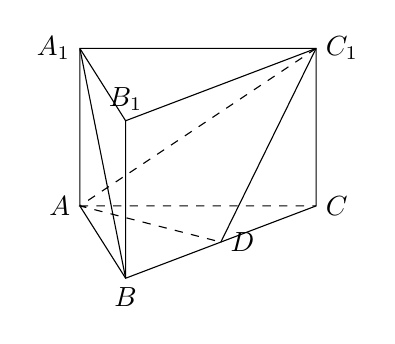
\begin{tikzpicture}
        \draw (0,0) node [left] {$A$} coordinate (A);
        \draw (3,0) node [right] {$C$} coordinate (C);
        \draw (1.5,0) ++ (225:{3/4*sqrt(3)}) node [below] {$B$} coordinate (B);
        \draw (A) ++ (0,2) node [left] {$A_1$} coordinate (A1);
        \draw (B) ++ (0,2) node [above] {$B_1$} coordinate (B1);
        \draw (C) ++ (0,2) node [right] {$C_1$} coordinate (C1);
        \draw (A) -- (B) -- (C) -- (C1) -- (A1) -- (A) (B) -- (B1) -- (A1) (B1) -- (C1);
        \draw ($(B)!0.5!(C)$) node [right] {$D$} coordinate (D);
        \draw (A1) -- (B) (D) -- (C1);
        \draw [dashed] (C1) -- (A) -- (D) (A) -- (C);
    \end{tikzpicture}
\end{center}
(1) 求证: 直线$A_1B$与$C_1D$为异面直线;\\
(2) 求三棱锥$B-AC_1D$的体积.
\item 已知代数式$(\dfrac 2m+\dfrac mx)^n$($m>0$, $x>0$).\\
(1) 当$m=2$, $n=6$时, 求二项展开式中二项式系数最大的项;\\
(2) 若$(\dfrac 2m+\dfrac mx)^{10}=a_0+\dfrac{a_1}x+\dfrac{a_2}{x^2}+\cdots +\dfrac{a_{10}}{x^{10}}$, 且$a_2=180$, 求$a_i$($0\le i \le 10$, $i\in \mathbf{N}$)的最大值.
\item 为实现``碳达峰'', 减少污染, 某化工企业开发了一个废料回收项目. 经测算, 该项目日回收成本$p$(元)与日回收量$x$(吨)($x\in [0,50]$)的函数关系可表示为$p=\begin{cases}20x, & 0\le x\le 30,  \\ x^2+16x-780, & 30<x \le 50,  \end{cases}$ 且每回收$1$吨废料, 转化成其他产品可收入$80$元.\\
(1) 设日纯收益为$y$元, 写出函数$y=f(x)$的解析式(纯收益$=$收入$-$成本);\\
(2) 该公司每日回收废料多少吨时, 获得纯收益最大?
\item 已知函数$f(x)=2^x+\dfrac a{2^x}$, $a$为实常数.\\
(1) 若函数$f(x)$为奇函数, 求$a$的值;\\
(2) 若$x\in [0,1]$时$f(x)$的最小值为$2$, 求$a$的值;\\
(3) 若方程$f(x)=6$有两个不等的实根$x_1,x_2$, 且$|x_1-x_2|\le 1$, 求$a$的取值范围.
\item 若实数$x,y\in [0,2\pi]$, 且满足$\cos (x+y)=\cos x+\cos y$, 则称$x$与$y$是``余弦相关''的.\\
(1) 若$x=\dfrac{\pi}2$, 求出所有与之``余弦相关''的实数$y$;\\
(2) 若存在实数$y$, 与$x$``余弦相关'', 求$x$的取值范围;\\
(3) 若不相等的两个实数$x$与$y$是``余弦相关''的, 求证: 存在实数$z$, 使得$x$与$z$ 为``余弦相关''的, $y$与$z$也为``余弦相关''的.


\item 函数$y=\sin (2x+\dfrac{\pi}3)$的最小正周期$T=$\blank{50}.
\item 已知集合$A=\{1,2,3,4\}$, $B=\{x|x\le \dfrac 52, \ x\in \mathbf{R}\}$, 则$A\cap B=$\blank{50}.
\item 已知函数$f(x)=\dfrac{x-1}{x+2}$的反函数为$f^{-1}(x)$, 则$f^{-1}(0)=$\blank{50}.
\item 若双曲线$x^2-\dfrac{y^2}m=1$的渐近线方程为$y=\pm 2x$, 则实数$m=$\blank{50}.
\item 在$(1+2x)^6$的二项展开式中, $x^2$项的系数为\blank{50}.
\item 已知圆锥的底面半径为$1$, 母线长为$3$, 则圆锥的体积为\blank{50}.
\item 已知复数$z$满足: $\mathrm{i}+\dfrac{2+\mathrm{i}}{\overline z}=0$($\mathrm{i}$为虚数单位), 则$|z|=$\blank{50}.
\item 方程$\log_3(x^2-1)=2+\log_3(x-1)$的解为$x=$\blank{50}.
\item 某市高考新政规定每位学生在物理、化学、生物、历史、政治、地理中选择三门作为等级考试科目, 则甲、乙两位学生等级考试科目恰有一门相同的不同选择共有
\blank{50}种(用数字作答).
\item 在$\triangle ABC$中, 三边$a$、$b$、$c$所对的三个内角分别为$A$、$B$、$C$, 若$a=3$, $b=2\sqrt 6$, $B=2A$, 则边长$c=$\blank{50}.
\item 在平面直角坐标系中, 已知点$A(-1,0)$、$B(0,3)$, $EF$为圆$x^2+y^2=4$上两个动点, 且$|\overrightarrow{EF}|=4$, 则$\overrightarrow{AE}\cdot \overrightarrow{BF}$的最大值为\blank{50}.
\item 无穷等差数列$\{a_n\}$满足: \textcircled{1} $a_1<0$, $a_2>\dfrac 32$; \textcircled{2} 在区间$(11,20)$中的项恰好比区间$[41,50]$中的项少$2$项, 则数列$\{a_n\}$的通项公式为$a_n=$\blank{50}.
\item 关于$x$、$y$的二元一次方程组$\begin{cases}x+2y=3, \\ 3x+4y=-1 \end{cases}$的增广矩阵为\bracket{20}.
\fourch{$\begin{pmatrix}1 & 2  \\3 & 4  \end{pmatrix}$}{$\begin{vmatrix} 1 & 2  \\3 & 4  \end{vmatrix}$}{$\begin{pmatrix} 1 & 2 & -3 \\ 3 & 4 & 1\end{pmatrix}$}{$\begin{pmatrix}1 & 2 & 3 \\ 3 & 4 & -1\end{pmatrix}$}
\item 记数列$\{a_n\}$的通项公式为$a_n=\begin{cases}
(-1)^n, &  n\le 2021,  \\ \dfrac{2n+1}{n+1}, &  n\ge 2022, \end{cases}$ $n\in \mathbf{N}^*$, 则数列$\{a_n\}$的
极限为\bracket{20}.
\fourch{$-1$}{$1$}{$2$}{不存在}
\item 如图, 在正方体$ABCD-A_1B_1C_1D_1$中, 点$MN$分别在棱$AA_1CC_1$上, 则``直线$MN\perp\text{直线}C_1B$''是``直线$MN\perp\text{平面}C_1BD$''的\bracket{20}.
\begin{center}
    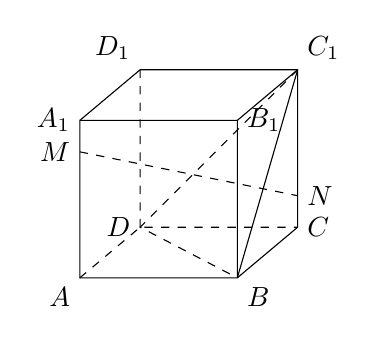
\begin{tikzpicture}
        \draw (0,0) node [below left] {$A$} coordinate (A) --++ (2,0) node [below right] {$B$} coordinate (B) --++ (40:{2/2}) node [right] {$C$} coordinate (C)
        --++ (0,2) node [above right] {$C_1$} coordinate (C1)
        --++ (-2,0) node [above left] {$D_1$} coordinate (D1) --++ (220:{2/2}) node [left] {$A_1$} coordinate (A1) -- cycle;
        \draw (A) ++ (2,2) node [right] {$B_1$} coordinate (B1) -- (B) (B1) --++ (40:{2/2}) (B1) --++ (-2,0);
        \draw [dashed] (A) --++ (40:{2/2}) node [left] {$D$} coordinate (D) --++ (2,0) (D) --++ (0,2);
        \draw ($(A)!0.8!(A1)$) node [left] {$M$} coordinate (M);
        \draw ($(C1)!0.8!(C)$) node [right] {$N$} coordinate (N);
        \draw [dashed] (M) -- (N)  (C1) -- (D) -- (B);
        \draw (B) -- (C1);
    \end{tikzpicture}
\end{center}
\twoch{充分非必要条件}{必要非充分条件}{充要条件}{既不充分又不必要条件}\item 已知非空集合$A,B$满足: $A\cup B=R$, $A\cap B=\varnothing$, 函数$f(x)=\begin{cases}
x^2, &  x\in A,  \\ 2x-1, &  x\in B.  \end{cases}$ 对于下列两个命题: \textcircled{1} 存在唯一的非空集合对$(A,B)$, 使得$f(x)$为偶函数; \textcircled{2} 存在无穷多非空集合对$(A,B)$, 使得方程$f(x)=2$无解. 下面判断正确的是\bracket{20}.
\fourch{\textcircled{1} 正确, \textcircled{2} 错误}{\textcircled{1} 错误, \textcircled{2} 正确}{\textcircled{1} 、\textcircled{2} 都正确}{\textcircled{1} 、\textcircled{2} 都错误}
\item 如图, 直三棱柱$ABC-A_1B_1C_1$的底面为直角三角形且$\angle ACB=90^\circ$, 直角边$CA$、$CB$的长分别为$3$、$4$, 侧棱$AA_1$的长为$4$, 点$M$、$N$分别为线段$A_1B_1$、$C_1B_1$的中点.
\begin{center}
    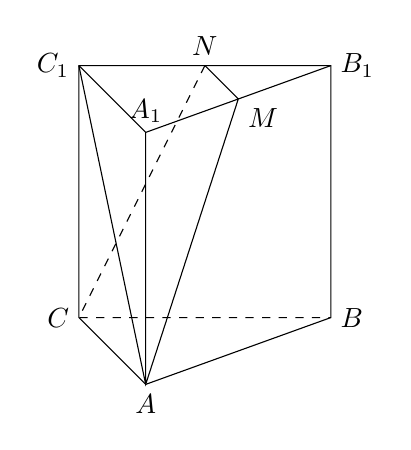
\begin{tikzpicture}[scale = 0.8]
        \draw (0,0) node [left] {$C$} coordinate (C);
        \draw (4,0) node [right] {$B$} coordinate (B);
        \draw (-45:1.5) node [below] {$A$} coordinate (A);
        \draw (A) ++ (0,4) node [above] {$A_1$} coordinate (A1);
        \draw (B) ++ (0,4) node [right] {$B_1$} coordinate (B1);
        \draw (C) ++ (0,4) node [left] {$C_1$} coordinate (C1);
        \draw ($(A1)!0.5!(B1)$) node [below right] {$M$} coordinate (M);
        \draw ($(C1)!0.5!(B1)$) node [above] {$N$} coordinate (N);
        \draw (A) -- (B) -- (B1) -- (C1) -- (C) -- cycle;
        \draw (C1) -- (A) -- (M) -- (N) (A1) -- (A) (A1) -- (C1) (A1) -- (B1);
        \draw [dashed] (N) -- (C) -- (B);
    \end{tikzpicture}
\end{center}
(1) 求证: $A,C,N,M$四点共面;\\
(2) 求直线$AC_1$与平面$ACNM$所成角的大小.
\item 已知函数$f(x)=\sin \omega x+\cos \omega x$.\\
(1) 若$\omega =2$, 求函数$f(x)$在$[0,\pi]$上的零点;\\
(2) 已知$\omega =1$, 函数$g(x)=(f(x))^2+\sqrt 3\cos 2x$, $x\in [0,\dfrac{\pi}4]$, 求函数$g(x)$的值域.
\item 为了防止某种新冠病毒感染, 某地居民需服用一种药物预防. 规定每人每天定时服用一次, 每次服用$m$毫克.已知人的肾脏每$24$小时可以从体内滤除这种药物的$80\%$, 设第$n$次服药后(滤除之前)这种药物在人体内的含量是$a_n$毫克, (即$a_1=m$).\\
(1)	已知$m=12$, 求$a_2$、$a_3$;\\
(2)	该药物在人体的含量超过25毫克会产生毒副作用, 若人需要长期服用这种药物, 求$m$的最大值.
\item 如图, 椭圆$C:\dfrac{x^2}{a^2}+\dfrac{y^2}{b^2}=1$($a>b>0$)的左、右焦点分别为$F_1$、$F_2$, 过右焦点$F_2$与$x$轴垂直的直线交椭圆于$MN$两点, 动点$P$、$Q$分别在直线$MN$与椭圆$C$上.已知$|F_1F_2|=2$, $\triangle MNF_1$的周长为$4\sqrt 2$.\\
\begin{center}
    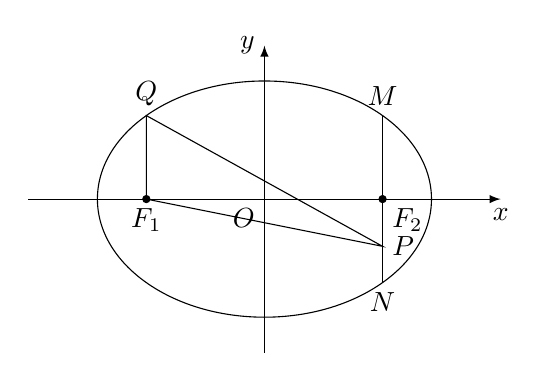
\begin{tikzpicture}[>=latex,scale = 1.5]
        \draw [->] (-2,0) -- (2,0) node [below] {$x$};
        \draw [->] (0,-1.3) -- (0,1.3) node [left] {$y$};
        \draw (0,0) node [below left] {$O$};
        \draw (0,0) ellipse ({sqrt(2)} and 1);
        \draw (1,{-sqrt(2)/2}) node [below] {$N$}-- (1,{sqrt(2)/2}) node [above] {$M$};
        \filldraw (-1,0) circle (0.03) node [below] {$F_1$} (1,0) circle (0.03) node [below right] {$F_2$};
        \draw (-1,0) -- (-1,{sqrt(2)/2}) node [above] {$Q$} -- (1,-0.4) node [right] {$P$} -- cycle;

    \end{tikzpicture}
\end{center}
(1)	求椭圆$C$的方程;\\
(2)	若线段$PQ$的中点在$y$轴上, 求三角形$F_1QP$的面积;\\
(3)	是否存在以$F_1Q$、$F_1P$为邻边的矩形$F_1PEQ$, 使得点$E$在椭圆$C$上? 若存在, 求出所有满足条件的点$Q$的横坐标; 若不存在, 说明理由.
\item 给定区间$I$和正常数$a$, 如果定义在$\mathbf{R}$上的两个函数$y=f(x)$与$y=g(x)$满足: 对一切$x\in I$, 均有$|f(x)-g(x)|\le a$, 称函数$y=f(x)$与$y=g(x)$具有性质$P(I,a)$.\\
(1)	已知$I=(0,+\infty)$, 判断下列两组函数是否具有性质$P(I,2)$? \textcircled{1} $f_1(x)=\dfrac 1{{x^2}+1}$, $g_1(x)=2$; \textcircled{2} $f_2(x)=x^2+x+1$, $g_2(x)=x^2-x+1$;(不需要说明理由)\\
(2)	已知$f(x)=0$, $y=g(x)$是周期函数, 且对任意的$a>0$, 均存在区间$I=(M,+\infty)$, 使得函数$y=f(x)$与$y=g(x)$具有性质$P(I,a)$, 求证: $g(x)=0$;\\
(3)	已知$I=[1,m]$, $f(x)=x^2$, 若存在一次函数$y=g(x)$与$y=f(x)$具有性质$P(I,1)$, 求实数$m$的最大值.

\item 已知$\overrightarrow a = (-1,1)$, 则$|\overrightarrow a|=$\blank{50}.
\item 函数$y=\log_2(x+1)$的反函数为\blank{50}.
\item 若直线$l_1:2x+my+1=0$与$l_2:y=3x-1$垂直, 则实数$m=$\blank{50}.
\item 已知$2+\mathrm{i}$($\mathrm{i}$是虚数单位)是实系数一元二次方程$x^2+px+q=0$的根, 则$p+q=$\blank{50}.
\item 已知$\sin x=\dfrac{3}{5}$, $x\in (\dfrac \pi 2,\pi)$, 则行列式$\begin{vmatrix}   \sin x & -1 \\ 1 & \sec x \end{vmatrix}$的值等于\blank{50}.
\item 已知$A=\{x|\dfrac 2 x>1\}$, $B=\{x|\log_2 (x-1)<1\}$, 则$A\cap B=$\blank{50}.
\item 在某次数学测验中, $5$位学生的成绩如下: $78,85,a,82,69$, 他们的平均成绩为$80$, 则他们的成绩的方差等于\blank{50}.
\item 已知实数$x,y$满足$\begin{cases}x+y\le 4, \\ y\ge x, \\ x\ge 1,\end{cases}$ 则$x+2y$的最大值为\blank{50}.
\item 若$(x+\dfrac 1{\sqrt{x}})^n$的二项展开式中各项系数的和等于$64$, 则其中$x^3$的系数是\blank{50}.
\item 三阶矩阵$\begin{pmatrix}
    a_{11} & a_{12} & a_{13} \\ a_{21} & a_{22} & a_{23} \\ a_{31} & a_{32} & a_{33}
\end{pmatrix}$中有$9$个不同的数$a_{ij}$($i=1,2,3$, $j=1,2,3$), 从中任取三个, 则至少有两个数位于同行或同列的概率是\blank{50}(结果用分数表示).
\item 已知抛物线$y^2=4x$, 斜率为$k$的直线$l$经过抛物线的焦点$F$, 与抛物线交于$P$、$Q$两点, 点$Q$关于$x$轴的对称点为$Q'$, 点$P$关于直线$x=1$的对称点为$P'$, 且满足$P'Q'\perp PQ$, 则直线$l$的方程为\blank{50}.
\item 若函数$f(x)=\cos mx$($m>0$)在区间$(2\pi,3\pi)$内既没有取到最大值$1$, 也没有取到最小值$-1$, 则$m$的取值范围为\blank{50}.
\item 设$x_1,x_2\in \mathbf{R}$, 则``$x_1+x_2>6$且$x_1x_2>9$''是``$x_1>3$且$x_2>3$''的\bracket{20}.
\twoch{充分不必要条件}{必要不充分条件}{充要条件}{既不充分也不必要条件}
\item 数列$\{a_n\}$为等差数列, $a_1>0$且公差$d>0$, 若$\lg a_1$, $\lg a_3$, $\lg a_6$也是等差数列, 则其公差为\bracket{20}.
\fourch{$\lg d$}{$\lg 2d$}{$\lg \dfrac 23$}{$\lg \dfrac 32$}
\item 椭圆$C:\dfrac{x^2}{4}+\dfrac{y^2}{3}=1$的左、右顶点分别为$A_1,A_2$, 点$P$在$C$上($P$不与$A_1,A_2$重合)且直线$PA_2$的斜率的取值范围是$[-2,-1]$, 那么直线$PA_1$斜率的取值范围是\bracket{20}.
\fourch{$[\dfrac 12,\dfrac 34]$}{$[\dfrac 38,\dfrac 34]$}{$[\dfrac 12, 1]$}{$[\dfrac 34,1]$}
\item 定义域为$[a,b]$的函数$y=f(x)$图像的两个端点为$A(a,f(a))$, $B(b,f(b))$. $M(x,y)$是$y=f(x)$图像上任意一点, 过点$M$作垂直于$x$轴的直线$l$交线段$AB$于点$N$(点$M$与点$N$可以重合), 我们称$|\overrightarrow{MN}|$的最大值为该函数的``曲径''. 下列定义域为$[1,2]$的函数中, 曲径最小的是\bracket{20}.
\fourch{$y=x^2$}{$y=\dfrac 2x$}{$y=x-\dfrac 1x$}{$y=\sin \dfrac\pi 3 x$}
\item 如图, 圆锥的顶点为$P$, 底面圆心为$O$, 线段$AB$和线段$CD$都是底面圆的直径, 且$AB\perp CD$, 取劣弧$BC$上一点$E$, 使$\angle COE=\dfrac\pi 3$, 连结$PE$. 已知$|OA|=1$, $|PA|=2$.
\begin{center}
    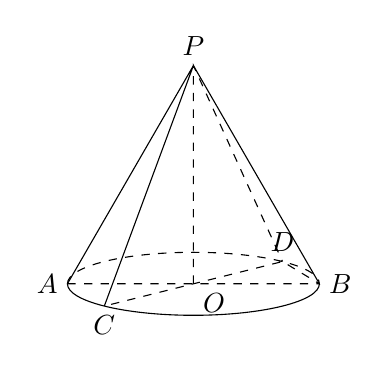
\begin{tikzpicture}[scale = 0.8]
        \draw (-2,0) node [left] {$A$} coordinate (A);
        \draw (2,0) node [right] {$B$} coordinate (B);
        \draw (0,0) node [below right] {$O$} coordinate (O);
        \draw (0,{2*sqrt(3)})node [above] {$P$} coordinate (P);
        \draw ({2*cos(225)},{0.5*sin(225)}) node [below] {$C$} coordinate (C);
        \draw ({2*cos(45)},{0.5*sin(45)}) node [above] {$D$} coordinate (D);
        \draw (A) arc (180:360:2 and 0.5) -- (P) -- (A) (P) -- (C);
        \draw [dashed] (A) arc (180:0:2 and 0.5) -- (D) -- (C) (A) -- (B) (O) -- (P) -- (D);
    \end{tikzpicture}
\end{center}
(1) 求该圆锥的体积;\\
(2) 求异面直线$PE$、$BD$所成角的大小.
\item 已知函数$f(x)=x^2+mx+3$, 其中$m\in \mathbf{R}$.\\
(1) 若不等式$f(x)<5$的解集是$(-1,2)$, 求$m$的值;\\
(2) 若函数$y=f(x)$在区间$[0,3]$上有且仅有一个零点, 求$m$的取值范围.
\item 如图, 有一块扇形草地$OMN$, 已知半径为$4$, $\angle MON=\dfrac\pi 2$, 现要在其中圈出一块举行场地$ABCD$作为儿童乐园使用, 其中点$A$、$B$在弧$\overset\frown{MN}$上, 且线段$AB$平行于线段$MN$.
\begin{center}
    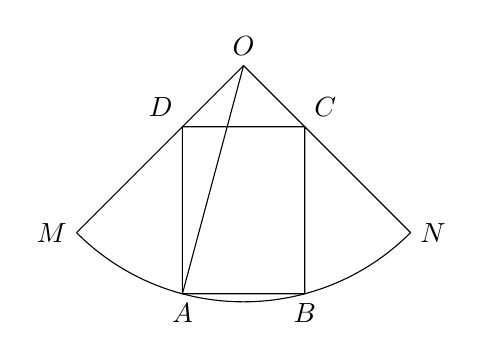
\begin{tikzpicture}[scale = 1.5]
        \draw (0,0) node [above] {$O$} coordinate (O);
        \draw (-45:2) node [right] {$N$} coordinate (N);
        \draw (-135:2) node [left] {$M$} coordinate (M);
        \draw (-75:2) node [below] {$B$} coordinate (B);
        \draw (-105:2) node [below] {$A$} coordinate (A);
        \draw (-45:{2/sin(45)*sin(15)}) node [above right] {$C$} coordinate (C);
        \draw (-135:{2/sin(45)*sin(15)}) node [above left] {$D$} coordinate (D);
        \draw (M) -- (O) -- (N) (A) rectangle (C) (O) -- (A);
        \draw (M) arc (-135:-45:2);
    \end{tikzpicture}
\end{center}
(1) 若点$A$为弧$\overset\frown{MN}$的一个三等分点, 求矩形$ABCD$的面积$S$;\\
(2) 当$A$在何处时, 矩形$ABCD$的面积$S$最大? 最大值为多少?
\item 已知椭圆$C:\dfrac{x^2}{a^2}+\dfrac{y^2}{b^2}=1$($a>b>0$), 过定点$T(t,0)$的直线交椭圆于$P,Q$两点, 其中$t\in (0,a)$.
\begin{center}
    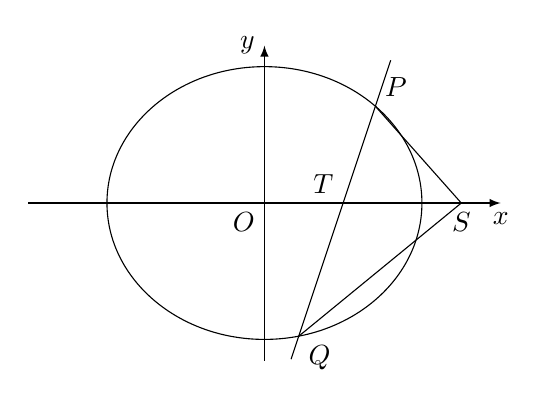
\begin{tikzpicture}[>=latex]
        \draw [->] (-3,0) -- (3,0) node [below] {$x$};
        \draw [->] (0,-2) -- (0,2) node [left] {$y$};
        \draw (0,0) node [below left] {$O$};
        \draw [name path = ell] (0,0) ellipse (2 and {sqrt(3)});
        \draw (1,0) node [above left] {$T$} coordinate (T);
        \path (0.4,-1.8) coordinate (U) ($(U)!2!(T)$) coordinate (V);
        \path [name path = line] (U) -- (V);
        \path [name intersections = {of = ell and line, by = {P,Q}}];
        \draw ($(P)!{-0.2}!(Q)$) -- (P) node [above right] {$P$} -- (Q) node [below right ] {$Q$} -- ($(Q)!{-0.1}!(P)$) ;
        \draw (2.5,0) node [below] {$S$} coordinate (S);
        \draw (P) -- (S) -- (Q);
    \end{tikzpicture}
\end{center}
(1) 若椭圆短轴长为$2\sqrt{3}$且经过点$(-1,\dfrac 32)$, 求椭圆方程;\\
(2) 对(1)中的椭圆, 若$t=\sqrt{3}$, 求$\triangle OPQ$面积的最大值;\\
(3) 在$x$轴上是否存在点$S(s,0)$使得$\angle PST=\angle QST$恒成立? 如果存在, 求出$s,t$的关系; 如果不存在, 说明理由.
\item 已知$a$为实数, 数列$\{a_n\}$满足: \textcircled{1} $a_1=a$; \textcircled{2} $a_{n+1}=\begin{cases}
a_n-3, & a_n>3, \\ 4-a_n, & a_n\le 3,\end{cases}$($n\in \mathbf{N}^*$). 若存在一个非零常数$T\in \mathbf{N}^*$, 对任意$n\in \mathbf{N}^*$, $a_{n+T}=a_n$都成立, 则称数列$\{a_n\}$为周期数列.\\
(1) 当$a=3$时, 求$a_1+a_2+a_3+a_4$的值;\\
(2) 求证: 存在正整数$n$, 使得$0\le a_n\le 3$;\\
(3) 设$S_n$是数列$\{a_n\}$的前$n$项和, 是否存在实数$a$满足: \textcircled{1} 数列$\{a_n\}$为周期数列; \textcircled{2} 存在正奇数$k$, 使得$S_k=2k$. 若存在, 求出所有$a$的可能值; 若不存在, 说明理由.

\item 若集合$A=(-\infty ,1)$, $B=(0,+\infty)$, 则$A\cap B=$\blank{50}.
\item 复数$z=2-\mathrm{i}$, 则$|z|=$\blank{50}.
\item 直线$l$的参数方程为$\begin{cases} x=2+t, \\ y=1+2t, \end{cases}$($t\in \mathbf{R}$), 则直线$l$的斜率为\blank{50}.
\item $(1+2x)^{10}$ 的二项展开式中, $x^2$ 项的系数为\blank{50}.
\item 若圆锥的母线长为$5$, 底面半径为$3$, 则该圆锥的体积为\blank{50}.
\item 函数$f(x)=1+\lg x$的反函数是$f^{-1}(x)$=\blank{50}.
\item 设$a,b,c,d\in \mathbf{R}$, 若行列式$\begin{vmatrix}    a & b & 1  \\ c & d & 2  \\ 0 & 0 & 3  \end{vmatrix}=9$, 则行列式$\begin{vmatrix} a & b  \\ c & d  \end{vmatrix}$的值为\blank{50}.
\item 已知集合$A=\{-2,-1,-\dfrac 12,\dfrac 13,\dfrac 12,1,2,3\}$, 从集合$A$中任取一个元素$a$, 使函数$y=x^a$是奇函数且在$(0,+\infty)$上递增的概率为\blank{50}.
\item 等差数列$\{a_n\}$的前$n$项和为$S_n$, 若$S_5=S_7$, 且$a_2+a_3=8$, 则$\displaystyle\lim_{n\to\infty}\dfrac{S_n}{n^2}=$\blank{50}.
\item 已知点$P$为正$\triangle ABC$边上或内部的一点, 且实数$x,y$满足$\overrightarrow{AP}=x\overrightarrow{AB}+2y\overrightarrow{AC}$, 则$x-y$的取值范围是\blank{50}.
\item 设点$P$是曲线$y=\sqrt{x^2+1}$上的动点, 点$F(0,-\sqrt 2)$, $A(\sqrt 2,0)$满足$|PF|+|PA|=4$, 则点$P$的坐标为\blank{50}.
\item 函数$f(x)=\cos \omega x$($\omega >0$, $x\in \mathbf{Z}$)的值域中仅有$5$个不同的值, 则$\omega$的最小值为\blank{50}.
\item ``$\alpha \in (0,\dfrac{\pi}2)$''是``$\alpha$ 为第一象限角''的\bracket{20}.
\twoch{充分不必要条件}{必要不充分条件}{充要条件}{既不充分又不必要条件}\item 下列不等式恒成立的是\bracket{20}.
\twoch{$|x+y|\ge |x-y|$}{$\sqrt{x^2+1}+x>0$}{$x+\dfrac 1x\ge 2$}{$|x+y|+|x-y|\le |x|+|y|$}
\item 上海入夏的标准为: 立夏之后, 连续五天日平均气温不低于$22^\circ\text{C}$. 立夏之后, 测得连续五天的平均气温数据满足如下条件, 其中能断定上海入夏的是\bracket{20}.
\twoch{总体均值为$25^\circ\text{C}$, 中位数为$23^\circ\text{C}$}{总体均值为$25^\circ\text{C}$, 总体方差大于$0^\circ\text{C}^2$}{总体中位数为$23^\circ\text{C}$, 众数为$25^\circ\text{C}$}{总体均值为$25^\circ\text{C}$, 总体方差为$1^\circ\text{C}^2$}
\item 对于定义在集合$D$上的两个函数$y_1=f_1(x)$与$y_2=f_2(x)$, 若对任意的$x\in D$, 总有$|f_2(x)|\le |f_1(x)|$成立, 则称函数$f_1(x)$包裹函数$f_2(x)$. 判断如下两个命题真假:\\
\textcircled{1}  函数$f_1(x)=kx$包裹函数$f_2(x)=x\cos x$的充要条件是$|k|\ge 1$;
\textcircled{2}  若对于任意$p>0$, $|f_1(x)-f_2(x)|<p$对任意$x\in D$都成立, 则函数$f_1(x)$包裹函数$f_2(x)$;\\
则下列选项正确的是\bracket{20}.
\fourch{\textcircled{1} 真, \textcircled{2} 假}{\textcircled{1} 假, \textcircled{2} 真}{\textcircled{1}、\textcircled{2} 全假}{\textcircled{1}、\textcircled{2} 全真}
\item 如图所示, 正四棱柱$ABCD-A_1B_1C_1D_1$的底面边长$1$, 侧棱长$4$, $AA_1$中点为$E$, $CC_1$中点为$F$.
\begin{center}
    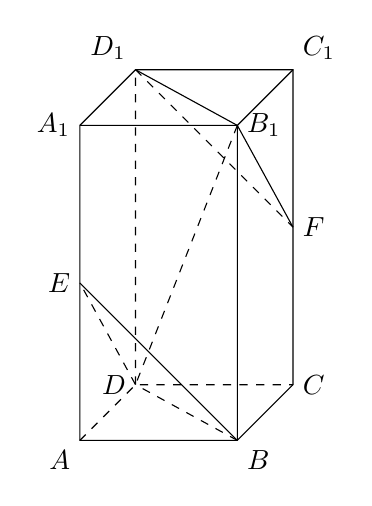
\begin{tikzpicture}
        \draw (0,0) node [below left] {$A$} coordinate (A) --++ (2,0) node [below right] {$B$} coordinate (B) --++ (45:{2/2}) node [right] {$C$} coordinate (C)
        --++ (0,4) node [above right] {$C_1$} coordinate (C1)
        --++ (-2,0) node [above left] {$D_1$} coordinate (D1) --++ (225:{2/2}) node [left] {$A_1$} coordinate (A1) -- cycle;
        \draw (A) ++ (2,4) node [right] {$B_1$} coordinate (B1) -- (B) (B1) --++ (45:{2/2}) (B1) --++ (-2,0);
        \draw [dashed] (A) --++ (45:{2/2}) node [left] {$D$} coordinate (D) --++ (2,0) (D) --++ (0,4);
        \draw ($(A)!0.5!(A1)$) node [left] {$E$} coordinate (E); 
        \draw ($(C)!0.5!(C1)$) node [right] {$F$} coordinate (F);
        \draw (B) -- (E) (D1) -- (B1) -- (F);
        \draw [dashed] (D1) -- (F) (B) -- (D) -- (E) (B1) -- (D);
    \end{tikzpicture}
\end{center}
(1) 求证: $\text{平面}BDE \parallel \text{平面}B_1D_1F$;\\
(2) 连结$B_1D$, 求直线$B_1D$与平面$BDE$所成的角的大小.
\item 已知函数$f(x)=t\sin x+|\cos x|$, 其中常数$t\in \mathbf{R}$.\\
(1) 讨论函数$f(x)$的奇偶性, 并说明理由;\\
(2) $\triangle ABC$中内角$A,B,C$所对的边分别为$a,b,c$, 且$a=2$, $b=\sqrt 5$, $f(A)=2$, 求当$t=\sqrt 3$时, $\triangle ABC$的面积.
\item 如图所示, 鸟类观测站需同时观测两处鸟类栖息地. $A$地在观测站正北方向, 且距离观测站$2$公里处, $B$地在观测站北偏东$\arcsin\dfrac 45$方向, 且距离观测站$5$公里. 观测站派出一辆观测车(记为点$M$)沿着公路向正东方向行驶进行观测, 记$\angle AMB$为观测角.
\begin{center}
    \begin{tikzpicture}
        \draw (-0.5,0) -- (3,0) node [below] {东};
        \draw (0,-0.5) -- (0,3) node [left] {北};
        \draw (0,0) node [below left] {观测站};
        \filldraw (0,1) circle (0.03) node [left] {$A$} coordinate (A);
        \draw (2,1.5) circle (0.03) node [above right] {$B$} coordinate (B);
        \draw (0.5,0) circle (0.03) node [below] {$M$} coordinate (M);
        \draw (A) -- (M) -- (B);        
    \end{tikzpicture}
\end{center}
(1) 当观测车行驶至距观测站$1$公里时, 求观测角$\angle AMB$的大小(精确到$0.1^\circ$);\\
(2) 为了确保观测质量, 要求观测角$\angle AMB$不小于$45^\circ$ , 求观测车行驶过程中满足要求的路程有多长(精确到$0.1$公里).\\
\item 如图, 中心在原点$O$的椭圆$\Gamma$ 的右焦点为$F(2\sqrt 3,0)$, 长轴长为$8$. 椭圆$\Gamma$上有两点$P,Q$, 连结$OP,OQ$, 记它们的斜率为$k_{OP}$、$k_{OQ}$, 且满足$k_{OP}\cdot k_{OQ}=-\dfrac 14$.
\begin{center}
    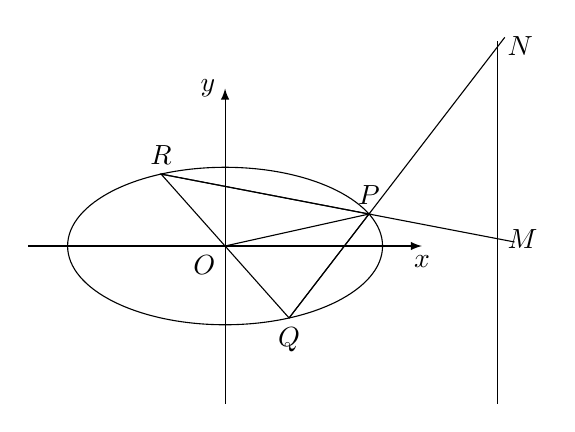
\begin{tikzpicture}[>=latex,scale = 0.5]
        \draw [->] (-5,0) -- (5,0) node [below] {$x$};
        \draw [->] (0,-4) -- (0,4) node [left] {$y$};
        \draw (0,0) node [below left] {$O$};
        \draw [name path = directrix] ({4*sqrt(3)},-4) -- ({4*sqrt(3)},5.2);
        \draw (0,0) ellipse (4 and 2);
        \draw ({4*cos(acos(sqrt(7)-sqrt(3)))},{2*sin(acos(sqrt(7)-sqrt(3)))}) node [above] {$P$} coordinate (P);
        \draw ({-4*sin(acos(sqrt(7)-sqrt(3)))},{2*cos(acos(sqrt(7)-sqrt(3)))}) node [above] {$R$} coordinate (R);
        \draw ({4*sin(acos(sqrt(7)-sqrt(3)))},{-2*cos(acos(sqrt(7)-sqrt(3)))}) node [below] {$Q$} coordinate (Q);
        \draw (0,0) -- (P) -- (R) -- (Q) -- (P);
        \draw [name path = line1] (Q) -- ($(Q)!2.7!(P)$);
        \draw [name path = line2] (R) -- ($(R)!1.7!(P)$);
        \draw [name intersections = {of = line1 and directrix, by = N}] (N) node [right] {$N$};
        \draw [name intersections = {of = line2 and directrix, by = M}] (M) node [right] {$M$};
    \end{tikzpicture}
\end{center}
(1)求椭圆$\Gamma$的标准方程;
(2)求证: ${{| OP |}^2}+{{| OQ |}^2}$为一定值, 并求出这个定值;
(3)设直线$OQ$与椭圆$\Gamma$的另一个交点为$R$, 直线$RP$ 和$PQ$分别与直线$x=4\sqrt 3$ 交于点$M,N$, 若$\triangle PQR$和$\triangle PMN$的面积相等, 求点$P$的横坐标.
\item 已知数列$\{a_n\}$满足: $a_1=1$, $a_{n+1}=-a_n$或$a_{n+1}=a_n+2$, 对一切$n\in \mathbf{N}^*$都成立. 记$S_n$为数列$\{a_n\}$的前$n$项和. 若存在一个非零常数$T\in \mathbf{N}^*$, 对于任意$n\in \mathbf{N}^*$, $a_{n+T}={a_n}$成立, 则称数列$\{a_n\}$为周期数列, $T$是一个周期.\\
(1) 求$a_2$、$a_3$所有可能的值, 并写出$a_{2022}$的最小可能值(不需要说明理由);\\
(2) 若$a_n>0$, 且存在正整数$p,q$($p\ne q$), 使得$\dfrac{a_p}q$与$\dfrac{a_q}p$均为整数, 求$a_{p+q}$的值;\\
(3) 记集合$S=\{n|S_n=0,n\in \mathbf{N}^*\}$, 求证: 数列$\{a_n\}$为周期数列的必要非充分条件为``集合$S$为无穷集合''.

\end{enumerate}
\end{document}